\begin{tabular}{c}
\begin{minipage}[c]{0.6\textwidth}
 \begin{exerciseS}[Corrente irrotazionale nel piano]
  Un flusso incomprimibile, irrotazionale, bidimensionale 
  e stazionario è descritto in coordinate polari dal potenziale cinetico
  \begin{equation*}
    \phi(r,\theta) = r^{2} cos(2 \theta)
  \end{equation*}
  Si chiede di:
  \begin{itemize}
    \item determinare il campo di velocità, eventuali punti di ristagno, 
          eventuali linee di corrente rettilinee;
    \item disegnare le linee di corrente;
    \item determinare il flusso attraverso il segmento che va dal punto 
          $A=(x_A,y_A)=
          (0,1)$ al punto $B=(x_B,y_B)=(1/\sqrt{2},1/\sqrt{2})$ e il 
          flusso attraverso l'arco di circonferenza centrata nell'origine,
          da $B$ a $C=(x_C,y_C)=(1,0)$. Discutere il risultato;
    \item dimostrare che le linee di corrente e le curve di livello del
          potenziale sono tra di loro perpendicolari.
  \end{itemize}
  \end{exerciseS}
\end{minipage}
\begin{minipage}[c]{0.35\textwidth}
   \begin{center}
   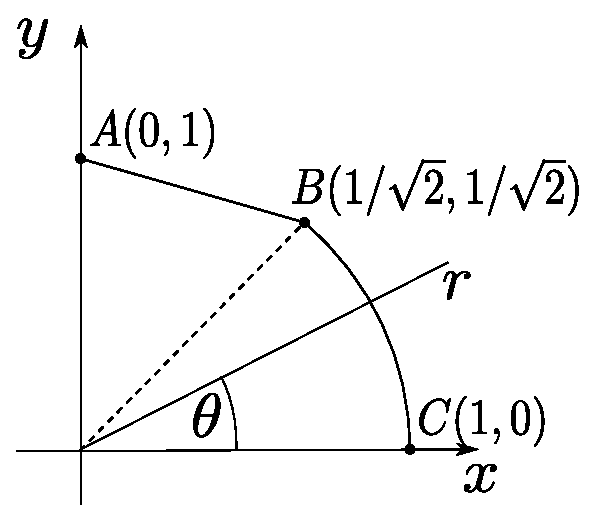
\includegraphics[width=1.00\textwidth]{./fig/piano2.eps}
   \end{center}
\end{minipage}
\end{tabular}

\sol

\partone
  Legame tra potenziale e velocità. Funzione di corrente per problemi 2D incomprimibili.
\begin{equation}
  \bm{u} = \bm{\nabla} \phi \quad
  \begin{cases}
  \begin{aligned}
   & u_x  =  \frac{\partial \phi}{\partial x}  = \frac{\partial \psi}{\partial y} \\
   & u_y  =  \frac{\partial \phi}{\partial y}  = - \frac{\partial \psi}{\partial x} \ .
  \end{aligned}
  \end{cases}
 \end{equation}
 Flusso di volume come differenza di funzione di corrente
 \begin{equation}
 \begin{aligned}
  \int_{A}^B \bm{u} \cdot {\bm{\hat{n}}} & =
  \int_{A}^B u n_x + v n_y = \\
 & = \int_A^B \dfrac{\partial \psi}{\partial x} t_x +
              \dfrac{\partial \psi}{\partial y} t_y = \\
 & = \int_A^B \left[ \dfrac{\partial \psi}{\partial x} \dfrac{dx}{ds} +
              \dfrac{\partial \psi}{\partial y} \dfrac{dy}{ds} \right] ds = \\
 & = \int_{A}^B \dfrac{d \psi}{ds} (x(s),y(s)) ds = \psi(B) - \psi(A) \ .
 \end{aligned}
\end{equation}

\parttwo

\begin{itemize}
 \item Campo di velocità, punto di ristagno e linee di corrente rettilinee
    \begin{itemize}
   \item  $\phi$, $\bm{u}$, $\psi$:
   \begin{equation*}
     \phi = r^2 \cos(2\theta) = r^2 ( \cos^2 \theta - \sin^2 \theta) = 
        x^2 - y^2
   \end{equation*}
   \begin{equation*}
    \begin{cases}
      u = \partial \phi / \partial x = 2x \\
      v = \partial \phi / \partial y = -2y
    \end{cases} \qquad \rightarrow \qquad  \psi(x,y) = 2 x y + C
   \end{equation*}
   
   \item punto di ristagno: $(x,y)=(0,0)$.
   \item Linee di corrente rettilinee: $(x,y) = (0,y)$ entranti nell'origine,
     $(x,y) = (x,0)$ uscenti dall'origine.
   \end{itemize}
 
 \item \dots
 \item flusso attraverso $AB$ e $BC$. La normale considerata ``punta a destra''
   mentre viene percorsa la curva: valgono quindi $n_x = t_y$ e $n_y = -t_x$.
   \begin{equation*}
    \begin{cases}
     \Phi_{AB} = \psi(B) - \psi(A) = 1 - 0 = 1  \\
     \Phi_{BC} = \psi(C) - \psi(B) = 0 - 1 = -1
    \end{cases}
   \end{equation*}
   Si consideri la curva chiusa costituita da $AB$, $BC$ e dagli assi. Non c'è
   flusso attraverso gli assi e quello che entra in $AB$ esce da $BC$. 
   \textit{il campo è regolare in tutto il dominio}.
 \item Il gradiente di una funzione è perpendicolare alle curve di livello: si
       può quindi verificare che i gradienti siano perpendicolari. Considerando
       le relazioni:
   \begin{equation*}
    \begin{cases}
      u & = \partial \phi / \partial x = \partial \psi / \partial y \\
      v & = \partial \phi / \partial y = - \partial \psi / \partial x
    \end{cases}
   \end{equation*}
   Si può scrivere
   \begin{equation*}
     \bm{\nabla}\phi \cdot \bm{\nabla}\psi = u v - v u = 0
   \end{equation*}
\end{itemize}



